\chapter{Subsystems}
\label{chap:subsystems}
.....



\section{Rover}
\label{sec:rover}
...
\section{Structure and Mechanics}
\label{sec:mechanics}
...
\section{Communications and Command and Data-Handling}
\label{sec:comm}
The Communications and C\&DH subsystem is responsible for the execution of Telecommand and Telemetry as well as payload data storing and transmission. Therefore the system consists of a pair of redundant Transmitter and Receiver as well as a redundant Single Board Computer OBC. The subsystem is located within the Electronic Bay.

\subsection{Communication System}
Requiring too many resources a direct link to earth has been deemed impractical. Instead communication for the INSPIRE mission is proposed to rely on a link between the rover and the Europa Lander. The lander then forwards data to earth via a satellite relay carrier which orbits the moon. The lander offers a $25\ dB$ high gain antenna [Missing Reference] and a low gain antenna which is not further specified in literature.\\

The downlink from the rover to the lander has been identified as the critical transmission path. However, link budget considerations reveal that a transmission to the LGA of the Europa Lander produces a link margin of $15.14\ dB$, resulting in a Bit Error Rate of less than $10^{-6}$.\\

Using the Landers LGA greatly increases robustness due to the elimination of pointing errors and higher margin for rover positioning error. Additionally, the INSPIRE rover’s communication link would not interfere with the Landers communication to the relay carrier by blocking the HGA. The link budget has been performed under the conservative considerations listed in Table [Missing Reference]. The complete link budget can be found in Appendix [Missing Reference]. 

\subsubsection{Component Selection}

Due to the considerably high link margin the focus is on low mass and low power components with flight heritage such as flown on CubeSat missions. Criteria with relatively small impact on the link budget such as component noise or even FEC have not been taken into account. Ideally the rover communication uses X-Band for increased compatibility with the lander and has a total system mass of less than $1\ kg$. \\
Since radiation hardness was not included in most datasheets a total dose of $<20\ krad$ was assumed in accordance with values for LEO [Missing Reference].

\subsubsection{Transmitter}

Since the transmission duty cycle is short, mass has become the design driving criteria followed by power. Output power is found sufficient in the $dBm$ regime. 
Subsequently the Transmitter Sputnix SXC-XTX-01 is selected for its low mass at $0.195\ kg$ and high data rate of up to $10\ Mbps$ [Missing Reference]. 

\subsubsection{Receiver}

Acting as the life line connection to mission control the receiver is required to run high duty cycles. Thus, low power consumption has become the design driving criteria followed by mass. Ultimately the Endurosat S-Band receiver is chosen due to its exceptional low power consumption of $2\ W$ and low mass of $0.220\ kg$ [Missing Reference]. However, as a S-Band receiver the device would have to be adapted which means an increase in rover design complexity.

\subsubsection{Antenna}

A set of four omnidirectional low gain antennas is positioned on the rover chassis to produce a half sphere coverage around the rover. Due to the high frequency, the antenna can be compact while remaining a passive component to save power. With mass being the dominating factor in the trade off the Endurosat X-Band single patch antenna with a mass of $2.2\ g$ seems fit [Missing Reference].

 \subsection{Command \& Data Handling}
 
 With respect to restricted power supply a redundant OBC hot-cold configuration stands to reason. Additionally, the standby mode is suggested during hibernation and charging modes relying solely on the PCDU (see chapter [Missing Reference]). 
Emphasis for the Electronics selection is placed on flight proven radiation hardness to increase mission robustness in the high radiation environment of the Jupiter system. 
Criteria of less importance are CPU speed and dimensions. \\

Instead of designing a new OBC board a trade-off was performed among existing single board computers. SBCs provide peripheral services such as bus interfaces, timer and memory in a flight proven configuration, which promises a simplified mission development. \\

BAE Systems provides a SBC with their flight proven Power PC750 Architecture which withstands a total radiation dose of up to $1\ Mrad$. The robustness comes at the cost of a $182\ MHz$ processor speed. \\

Additionally a custom housekeeping board will be tasked with providing engine control peripherals and sensor read out electronics.  

\section{Payload}
\label{sec:payload}
...

%-------------------------------------------------------------------------------
\section{Electrical Power System}
%-------------------------------------------------------------------------------
\label{sec:EPS}
The EPS (Electrical Power System) is the subsystem responsible for the electrical power supply of INSPIRE. It consists of four funadmental parts, which are the energy source, the PCDU unit (Power Control and Distribution) and the Energy Storage as well as the rover subsystems as the consumers. The EPS is visualized in \autoref{fig:epsflowchart}.

\begin{figure}[htb]
{\centering
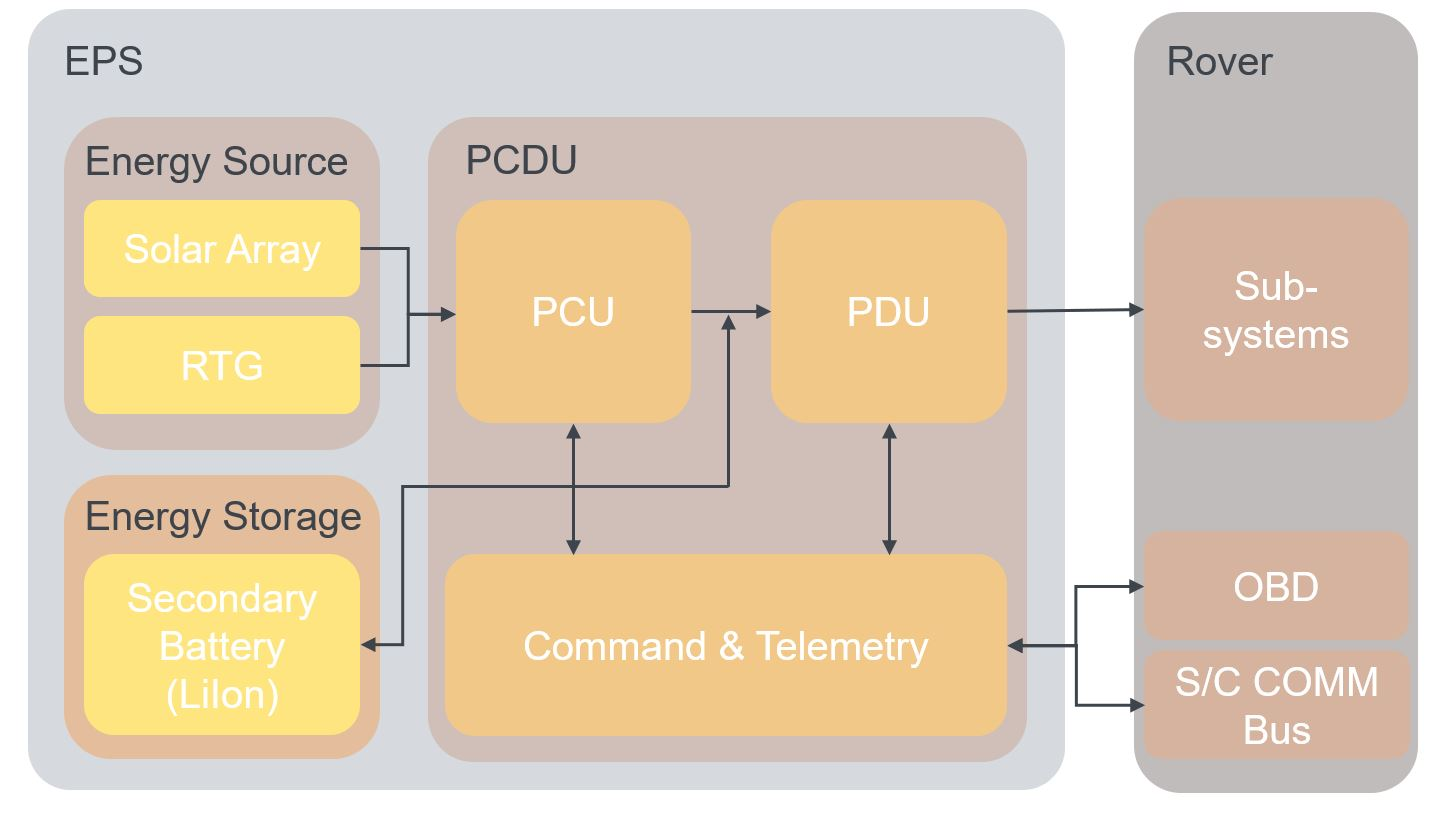
\includegraphics[width=0.7\textwidth]{Media/epsflowchart}
\caption{Functional Flow Chart Diagram for the EPS Subsystem.}
\label{fig:epsflowchart}
}
\end{figure}


\subsection{EPS Budget and Overview}
\autoref{tab:powbud} summarizes the power budget of INSPIRE based on the rover system modes defined in \autoref{chap:rovsubmod}. The complete power budget can be found in \autoref{tab:powerbudgetcomplete}.
As can be seen, the Locomotion mode has the highest demands on the EPS. Communication mode also has a high consumption. However, since this is primarily used at night and the rover can be charged again afterwards without any problems, it does not place any major restrictions on the power budget. Idle/Perception mode has a low consumption, but is usually used for a long time at a stretch and therefore also places high demands on the EPS. In Charging mode, the EPS is able to charge $7.04 \ W_{el} $.


\begin{table}[htb]
\centering
\begin{tabular}{|c|c|}
\hline
\textbf{Rover System Mode} & \textbf{\begin{tabular}[c]{@{}c@{}}Total Rover \\ Power Demand \\ including battery charge $P_\text{mode}$ [$W_{el}$]\end{tabular}} \\ \hline
Idle/Perception            & $15.25$                                                                                                                             \\ \hline
Safe/Hibernation           & $-5.84$                                                                                                                             \\ \hline
Communication              & $36.92$                                                                                                                             \\ \hline
Charging                   & $-7.04$                                                                                                                             \\ \hline
Locomotion                 & $232.36$                                                                                                                            \\ \hline
Payload: Observation       & $15.41$                                                                                                                             \\ \hline
Payload: Ice Core Mode     & $9.77$                                                                                                                              \\ \hline
\end{tabular}
\caption{Overview of the Power Budget of INSPIRE.}
\label{tab:powbud}
\end{table}


\subsection{Energy Source}
For the energy generation of INSPIRE many possible sources were taken into consideration for a trade-off. As a conclusion of this trad-off the decision was made to utilize a Radioisotope Thermoelectric Generator (RTG) as the main energy source for INSPIRE.\\
As the research couldn't find an RTG with a mass suitable for INSPIRE, the solution was to scale down a bigger RTG as an approximation. As a baseline of the scaling the eMMRTG (Enhanced Multi Mission Radioisotope Thermoelectric Generator) was utilized, which is currently under development at NASA and is especially designed for deep space missions like Europa. For the scaling a goal RTG mass of $m_\text{RTG}=3 \ \text{kg}$ was defined and the eMMRTG was scaled down using the given data.\\
In \autoref{tab:esmmrtg} the scaling results for the eSMMRTG (Enhanced and Scaled Multi Mission Radioisotope Thermoelectric Generator) are listed. The eSMMRTG has a BOL specific power of $\alpha_\text{BOL}= 4.0 \ \frac{W_{el}}{kg}$ and provides an electrical power of $P_{el} = 12.08 \ W_{el}$ during the mission duration\cite{R.Abelsonetal..2004}\cite{S.Magdum.2019}\cite{Holgate.2015}\cite{eMMRTG.NASA}\cite{Lakdawalla.2018}.



%The outcome of this trade-off is shown in \autoref{fig:epssourcetradeoff} for the most promising energy sources. 

%
%\begin{figure}[htb]
%{\centering
%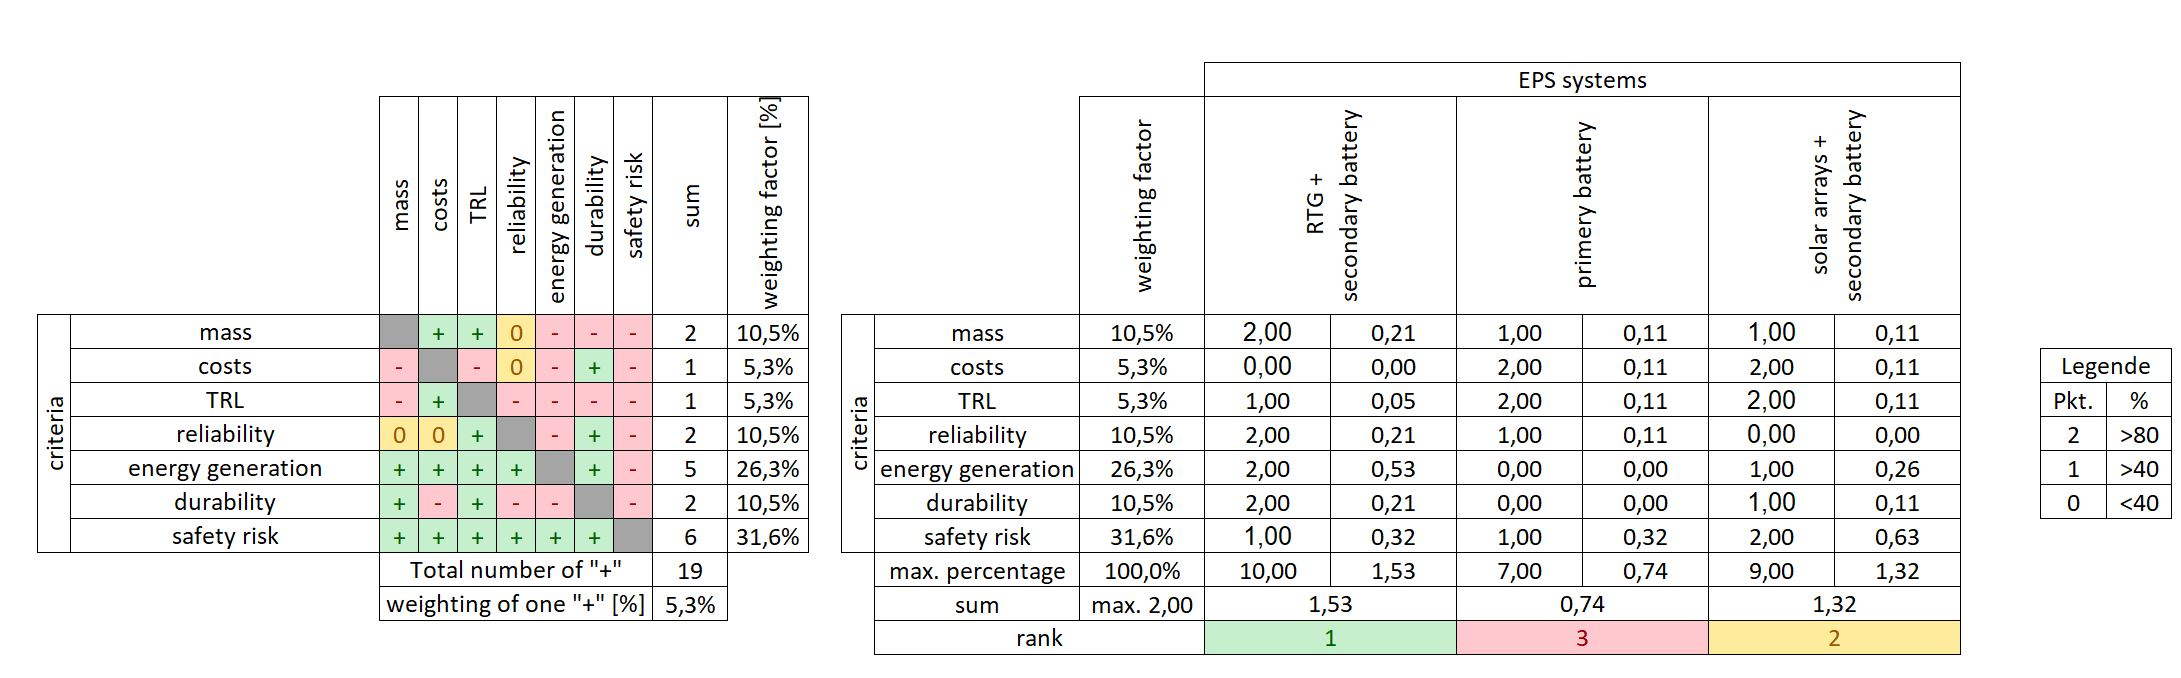
\includegraphics[width=0.7\textwidth]{Media/epssourcetradeoff}
%\caption{Trade-Off Conclusion for the EPS Energy Source.}
%\label{fig:epssourcetradeoff}
%}
%\end{figure}

\begin{table}[H]
\centering
\begin{tabular}{|c|c|}
\hline
\multicolumn{2}{|c|}{Scaled eSMMRTG Parameter}                \\ \hline
\textbf{System Mass} $m_\text{RTG}$ [$kg$]                             & \textbf{3.5}     \\ \hline
BOL Specific Power $\alpha_\text{BOL}$ $\frac{W_{el}}{kg}$  & $4.0$     \\ \hline
BOL Power $P_{el,\text{BOL}}$ $\ W_{el}$                    & $14$       \\ \hline
Isotrop                                                     & Pu-238   \\ \hline
Isotrop Half-Life [$a$]                                       & $87.7$     \\ \hline
Flight time and Storage (incl. Margins) [$a$]                 & $7$        \\ \hline
Power Loss Degradation until BOM $\ W_{el}$                 & $0.56$     \\ \hline
BOM Power $P_{el,\text{BOM}}$ $\ W_{el}$                    & $13.44$    \\ \hline
Europa Day Duration [$h$]                                     & $85$       \\ \hline
Mission Duration [$d$]                                        & $106.25$   \\ \hline
End of Mission Power $P_{el,\text{EOM}}$ [$\ W_{el}$]         & $13.42$   \\ \hline
\textbf{Final Power for Study} $P_{el}$ [$\ W_{el}$] (incl. $10\%$ scaling Margin) & \textbf{12.08}    \\ \hline

\end{tabular}
\caption{Parameters for the scaled eSMMRTG based on the eMMRTG.}
\label{tab:esmmrtg}
\end{table}

Furthermore INSPIRE will also be equipped with some radiation hardend solar arrays as already explained in \autoref{subsec:radhard}\cite{FraunhoferInstituteforSolarEnergySystemsISE.2021}. Since these solar cells are primarily used for technology testing, the mission must also be able to operate completely without this generated energy. For this reason, and because the expected energy generated by the solar cells is minimal, only the energy generated by the RTG is considered for the Phase 0 Study. However, it should be noted that these solar cells will also generate a certain amount of energy, which will benefitial for the EPS.


\subsection{Energy Storage} 
For the energy storage of INSPIRE many possible battery types were taken into consideration for a trade-off. As a conclusion of this trad-off the decision was made to utilize LiIon batteries as the secondary batteries of INSPIRE. This decision is primarly based on LiIon batteries high energy density, temperature range, robust performance and long operating and cycle life in extreme environments\cite{IRSatUniversityofStuttgart.2020}. \\
As the RTG only generates a small constant power the main energy source during the mission will be the accumulated energy of the batteries. The rover will charge the batteries at night, so the next exploration day can start with full capacity. Furthermore the batteries have to be charged during day time to maintain operations.\\
For the sizing of the batteries, the rover motion was chosen as the design driver, since this is the highest energy consuming state of the rover and additionally mission critical for INSPIRE. The rover motion consists of an interaction of the Locomotion and Perception mode as already mentioned in \autoref{chap:Operation}. Therefore it was defined that INSPIRE shall be able to drive $ 50 \ m $ (including alternating Locomotion and Perception Mode) with a fully charged Battery. The required battery capacity $C_\text{Batt,req}$ can be caculated using \autoref{eq:batreq}. The results are listed in \autoref{tab:batsize} \cite{S.Klinkner.2021}.


\begin{equation}
C_\text{Batt,req} = \frac{P_\text{el,req} \cdot t_e }{DoD \cdot \eta_\text{LiIon}}
\label{eq:batreq}
\end{equation}

\begin{table}[htb]
\centering

\begin{tabular}{|l|c|c|}
\hline
\textbf{Power Consumption Mode:}                        & \textbf{Locomotion} & \textbf{Perception} \\ \hline
Required Electrical Power $P_\text{el,req}$ [$W_{el}$]         & 283.43              & 14.01               \\ \hline
Duration of the mode $t_e$ [$s$]                          & 500              & 15000            \\ \hline
$DOD$ for Dimensioning [-]                              & 0.90                & 0.90                \\ \hline
Efficiency of LiIon Cells $\eta_\text{LiIon}$ [-]       & 0.95                & 0.95                \\ \hline
Required Battery Capacity per mode $C_\text{mode}$ [$Wh$] & 46.04               & 68.27               \\ \hline
\textbf{Total Required Battery Capacity} $C_\text{Batt,req}$ [$Wh$]    & \multicolumn{2}{c|}{\textbf{114.32}}               \\ \hline
\end{tabular}

\caption{Power consumption mode used as design case for the battery sizing.}
\label{tab:batsize}
\end{table}

Using these values a suitable battery cell and battery design configuration were conducted. Under consideration of these parameters the battery capacity $C_\text{Batt}$ can be calcuated:

\begin{equation}
C_\text{Batt} = C_\text{cell} \cdot V_\text{cell} \cdot N \cdot M .
\label{eq:batuse}
\end{equation}

According to the ECSS reliability restrictions 1 battery string must be substracted for dimensionsing. Furthermore a $30 \%$ margin on the energy content was applied. This leads to a final battery configuration with a capacity of $C_\text{Batt}=138,88 \ Wh$ and a mass of $m_\text{Batt} = 1980 \ g$. The final battery values are listed in \autoref{tab:battery} \cite{SAFTBatteries.2018}.


\subsection{EPS Power Control and Distribution}
In order to ensure the full functionality of the EPS, the last main component to be selected is a suitable PCDU. As described in \autoref{fig:epsflowchart}, the PCDU forms the heart of the EPS and is an important interface to the OBC and COMM. Furthermore the PCDU shall be able to monitor and control the rover system if necessary through watchdogs, HPC (High Priority Commands) and direct connections to the OBC and COMM.\\
The PCDU has the challenging task not only to process the RTG as the main energy source, but also to process solar cells as secondary energy sources. Therefore, a PCDU was sought which has the required size, dimensions and range of functions. The research resulted in the Nova PCDU from Bradford DSI. In addition, margins were added to the PCDU to ensure feasibility\cite{BradfordSpace.2019}.

\clearpage
%-------------------------------------------------------------------------------
\section{Radiation} \label{sec:Radiation}
%-------------------------------------------------------------------------------

Compared to the radiation environment near Earth the radiation environment near Jupiter is multiple times stronger. It has the highest radiation levels of any planet in our solar systems \cite{Platzhalter}. In order to survive these harsh environmental conditions, special emphasis must be placed on the radiation protection. In \autoref{fig:trappedprotonelectronfluxes}, the average trapped proton and electron fluxes on Europa's orbit around Jupiter are shown in comparison to the outer Van Allen radiation belt around Earth. However, in contrast to the Van Allen radiation belt, the duration within the radiation environment on Europa cannot be minimised and the rover has to be designed to withstand the entire mission duration of 30 days. \\ \\
In oder to design and evaluate different radiation protection approaches, different calculations have to be performed. For this purpose the ESA SPace ENVironment Information System (SPENVIS) is used \cite{Platzhalter}. All calculations and figures in \autoref{sec:Radiation} are performed with SPENVIS unless otherwise stated.

\subsection{Radiation Protection}

\label{subsec:RadiationProtection}

Various options are available to protect the rover against the radiation. A common approach is the use of aluminium or titanium as these materials can also act as structural elements. However, due to the mass constraints of 30 kg other materials or material compositions are taken in consideration which are more mass effective. In \autoref{tab:OptimalRadiationProtection}, an optimised shield structure is presented for different weight thresholds designed for the radiation environment around Jupiter.

\begin{wraptable}{r}{8cm}
\centering
\caption{Optimal shield structure for an Jupiter mission. \cite{Platzhalter}}
\begin{adjustbox}{max width=\textwidth}
\begin{tabular}[l]{cccccc}

	\toprule
	
	Areal Density	&	\(0.5\)	&	\(1\) &  \(2\) & \(3\)	\\
	/ \(\text{g/cm}^2\)	&	&	&  & \\
	
	\midrule
	
	
	Layer No. 1	&	Pb &  Pb & W	& Ta	\\
	/ mm	&	0.415 &  0.829 & 0.984	& 1.563	\\
	
	
	Layer No. 2	&	Fe	&  Mg &	Mg & Al \\
	/ mm	&	\(0.033\)	&  \(0.158\) &	\(0.540\) & \(0.399\) \\
	
	
	Layer No. 3 &	-	&  -	& - & Mg \\
	/ mm &	-	&  -	& - & \(0.150\) \\
	

	\bottomrule

\end{tabular}
\end{adjustbox}
\label{tab:OptimalRadiationProtection}
\end{wraptable}

The difference between an aluminium or titanium shielding and an optimised structure listed in \autoref{tab:OptimalRadiationProtection} for the total ionizing dose (TID) is shown in \autoref{fig:AluminiumTitanOptimised}. \\ \\
Due to the mass savings of the optimised structure it will be used where the radiation protection of the aluminium structure is not sufficient. In order to reduce the mass further, a radiation vault is utilised that highly sensible components do not have to be shielded separately.

\subsection{Components}

\label{subsec:RadiationComponents}

Every component on the rover has a different radiation tolerance and therefore have to be placed at different compartments within the rover. The radiation tolerances are listed in \autoref{tab:RadiationList}. None sensitive components like the electric motors and harness are only shielded by an aluminium structure where components like the metal within the wire are resistant against the radiation. However, isolators around the cables have to be selected to be resistant in order to prevent short circuits. Highly sensitive components like cameras have an additional protective layer in order to reduce the TID to under 30 krad. Components which are within the rover like the on-board computer (OBC) are placed within the radiation vault which reduces the TID to under 20 krad. For this purpose the optimised shield structure with a weight target of 0.5 \(\text{g/cm}^2\) is used. Detailed TIDs for all components are shown in \autoref{fig:CompartmentTID}.

\subsection{Improvements}

\label{subsec:RadiationImprovements}

Even though the radiation protection is sufficient for the rover to survive at least the nominal mission of 30 days, further improvements can be performed in order to extend the secondary mission. \\ \\
Local shielding can be applied on less resistant components in order to reduce the wall thickness of the whole radiation wall. If components with a radiation tolerance under 43.27 krad are individually shielded a mass saving of 736.2 g can be achieved. Additionally, water ice extracted from the surface of Europa can be used to improve the radiation protection. With a layer of one centimetre of water, the TID within the radiation vault can be reduced to 16.03 krad without the additional radiation protection beside the 4 mm of aluminium structure. The start mass of the rover can therefore be reduced by 897.2 g by removing the additional shielding. \\ \\
Detailed calculations for local shielding and water improvements can be found in \apprefsub{app:AppendixRadiationImprovements} and may be analysed further in Phase B.

\subsection{Conclusion}

\label{subsec:RadiationConclusion}

In order to protect the rover against the high radiation levels at the surface of Europa, the rover has different compartments. High sensible components are placed within a radiation vault which has a mass optimised structure. Components which has to be outside the radiation vault but are highly sensible are shielded individually. Low sensible Components are protected by the Aluminium structure. \autoref{fig:RadiationOverview} illustrates the different compartments within the rover and the accorded TIDs.

\begin{figure}[htb]
     \centering
     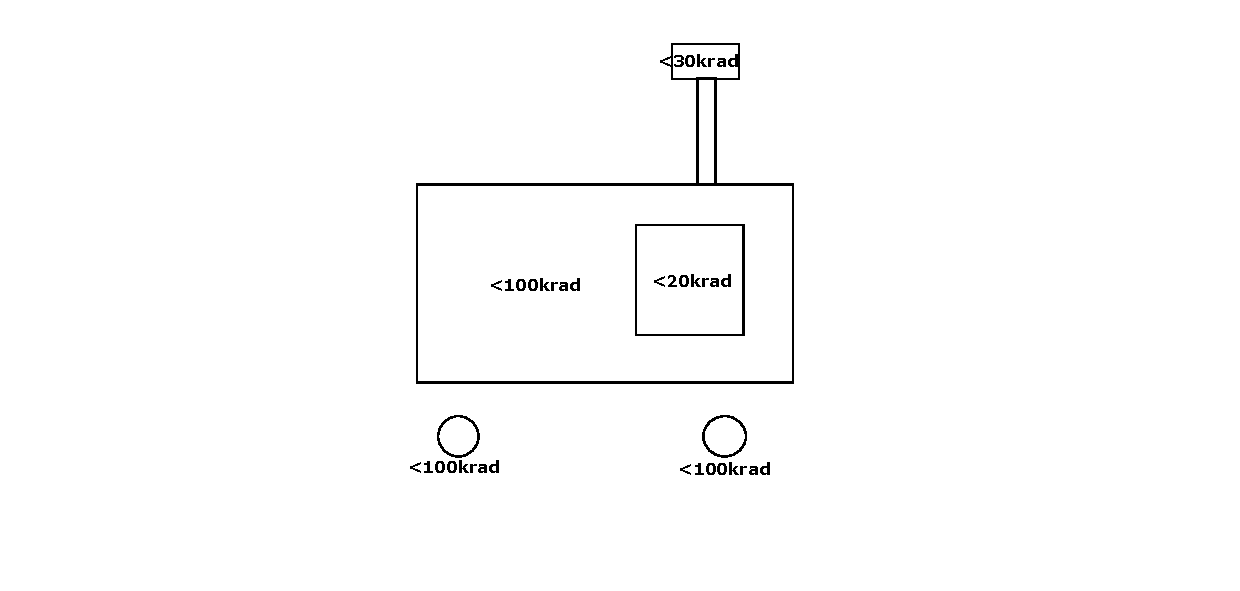
\includegraphics[width=\textwidth]{Media/RadiationOverview}
     \caption{Overview of TIDs within different compartments within the rover.}
     \label{fig:RadiationOverview}
\end{figure}

\clearpage

%-------------------------------------------------------------------------------
\section{Locomotion} \label{sec:locomotion}
%-------------------------------------------------------------------------------

The locomotion subsystem deals with the aspect of how the rover moves and the technical design, including the selection of components such as motors or gearboxes. Before the components can be determined, however, it is necessary to consider certain parameters and design drivers. These will be introduced in the following, and the decisions or estimations concerning the rover will be presented.

\subsection{Design drivers for Rover Classification}
\label{sec:DesignDriversLoco}

The first consideration in designing a rover is the environmental and operational conditions expected for the mission operation. The ice moon can be assumed to have a solid surface; thus, a wheeled rover is chosen. Further design drivers that led to the locomotion mobility systems are based on a tradeoff presented a tradeoff in \autoref{fig:TradeOffLoco}. However, the main design drivers are briefly summarised in \autoref{tab:Design Drivers Rover Movement}.

\begin{table}[htb]
\centering
\caption{Design Drivers for the rover movement technique regarding the environmental conditions on Europa and operating conditions.}
\label{tab:Design Drivers Rover Movement}
\resizebox{\textwidth}{!}{%
\begin{tabular}{|l|l|}
\hline
\rowcolor[HTML]{B3BBD1} 
\multicolumn{1}{|c|}{\cellcolor[HTML]{B3BBD1}Wheeled System}                                                                                                                     & \multicolumn{1}{c|}{\cellcolor[HTML]{B3BBD1}4-Wheels}                                                                                                \\ \hline
\begin{tabular}[c]{@{}l@{}}One of the most common types of platform\\ - high level of experience\\ - high TRL\end{tabular}                                                       & \begin{tabular}[c]{@{}l@{}}Compared to 2-wheels:\\ - stability  can be ensured \(\rightarrow\) important for drilling\\ - MMP decreases\end{tabular} \\ \hline
\begin{tabular}[c]{@{}l@{}}Compared to other systems:\\ - analysis quite straightforward\\ - simplification \(\rightarrow\) one of the most critical design drivers\end{tabular} & \begin{tabular}[c]{@{}l@{}}Compared to 6-wheels:\\ - less complex \(\rightarrow\) simplification\\ - mass can be reduced\end{tabular}                \\ \hline
\rowcolor[HTML]{B3BBD1} 
\multicolumn{1}{|c|}{\cellcolor[HTML]{B3BBD1}All-Wheel Drive}                                                                                                                    & \multicolumn{1}{c|}{\cellcolor[HTML]{B3BBD1}All-Wheel Actuation}                                                                                     \\ \hline
\begin{tabular}[c]{@{}l@{}}- traction can be increased\\ - increase of \(DP\) and the slope angle \(\theta\)\end{tabular}                                                        & - reduces the risk of slippage on ice                                                                                                                \\ \hline
\end{tabular}%
}
\end{table}

With the configured rover, the resulting wheel formula is 4 x 4 x 4. The normal force on Europa can be calculated to:

\begin{equation}
	W \:  = \:	m_\text{total} \cdot g_\text{Europa} \:  = \: 39.45 \, \text{N} \, 	.
	\label{eq:}
\end{equation}

Since each wheel is individually driven and controllable, the parameters in the following are designed for one wheel; the normal force per wheel is correspondingly \(W_\text{wheel} = 9.8625 ~\)N

\subsection{System Parameters}
\label{sec:SystemParametersLoco}

Regarding techniques of rover movement, it is crucial to consider the local conditions in which the rover will be operating. The surface of Europa can be assumed to be mainly covered by ice. However, since there are also geysers that transport water to the surface, surface areas may be covered by snow. Though Europa's surface temperature does not exceed 130 K, rather icy, hard-packed snow can be assumed. For this study, a conservative design of the rover is considered, whereby material parameters of snow in Sweden were selected, shown in \autoref{fig:SoilParameters}. Furthermore, the parameters depend on the width and diameter of the wheels of the rover. Therefore, several sizes dependent on the respective weight were selected and a limit per wheel was set to 200 g, illustrated in \autoref{fig:DimensionsLoco}. 

This constraint results in 6 configurations considered for the Rover system design, listed in \autoref{tab:Configurations}.

\begin{table}[htb]
\centering
\caption{Configurations for Rover Classification respective to the wheel width \(b\text{w}\), wheel diameter \(d_\text{w}\) and weight per wheel \(m_\text{w}\)}
\begin{adjustbox}{max width=\textwidth}
\begin{tabular}[l]{lccc}

	\toprule
		\multicolumn{1}{l}{Configuration} & \multicolumn{1}{c}{\(b\text{w}\) /m} & \multicolumn{1}{c}{Diameter \(d_\text{w}\) /m} & \multicolumn{1}{c}{Weight \(m_\text{w}\) /kg}   \\

	\midrule
		
		1	&	0.05	&	0.1		&	0.127		\\	
		2	&	0.06	&	0.1		&	0.153		\\
		3	&	0.07	&	0.1		&	0.178		\\
		4	&	0.05	&	0.125	&	0.154		\\
		5	&	0.05	&	0.125	&	0.185		\\
		6	&	0.05	&	0.15	&	0.185		\\

	\bottomrule

\end{tabular}
\end{adjustbox}
\label{tab:Configurations}
\end{table}




\subsubsection*{Mean Maximum Pressure}
\label{sec:MMP}



\begin{figure}[htb] 
  \centering
     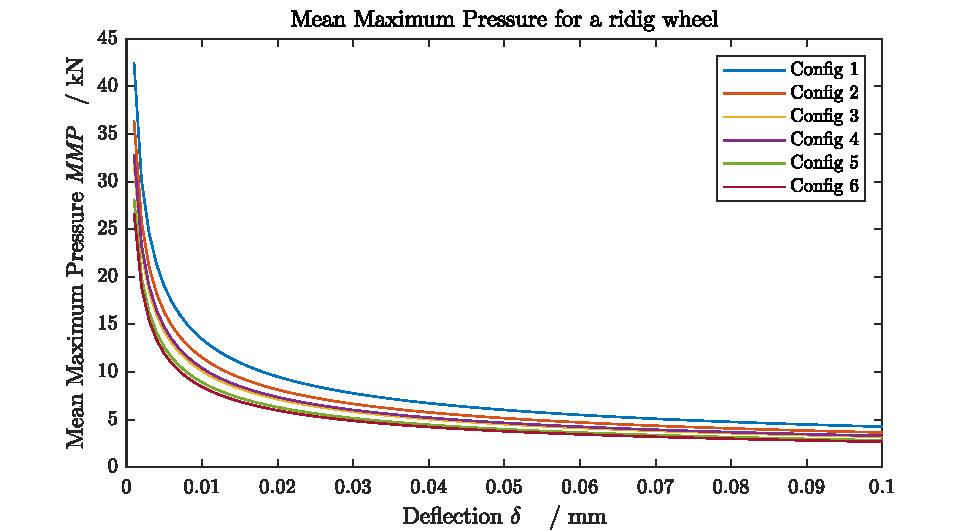
\includegraphics[width=1\textwidth]{Media/MMP for each Config.pdf}
  \caption{}
  \label{fig:}
\end{figure}

\subsubsection*{Drawbar Pull}
\label{sec:DP}



\begin{figure}[htb] 
  \centering
     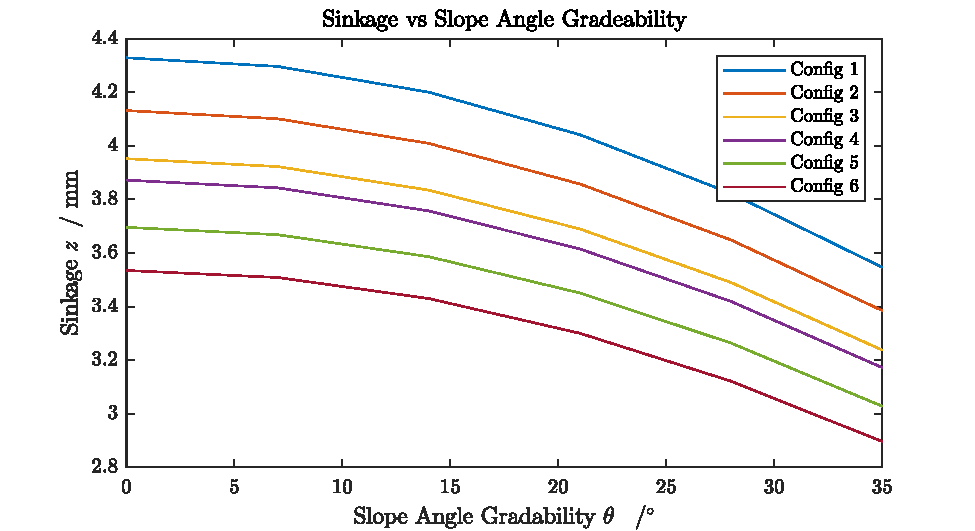
\includegraphics[width=1\textwidth]{Media/Sinkage for each config.pdf}
  \caption{}
  \label{fig:}
\end{figure}

\begin{figure}[htb] 
  \centering
     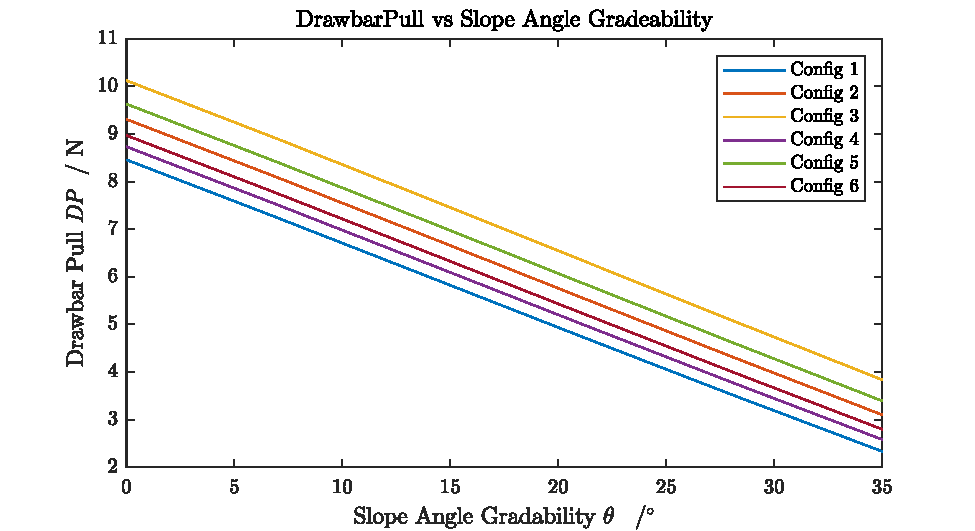
\includegraphics[width=1\textwidth]{Media/Drawbarpull for each Config.pdf}
  \caption{}
  \label{fig:}
\end{figure}





\subsubsection*{Steering}
\label{sec:Steering}



\subsubsection*{Hardware Selection}
\label{sec:HardwareLoco}



\subsection{Deployment mechanism}

%-------------------------------------------------------------------------------
\section{Control and Autonomy} \label{sec:ControlandAutonomy}
%-------------------------------------------------------------------------------



\clearpage
%-------------------------------------------------------------------------------
\section{Thermal Control System} \label{sec:thermalcontrol}
%-------------------------------------------------------------------------------
The main object of the Thermal Control System (TCS) is to keep the eletric components within their temperature limits, listed in \autoref{tab:tcs_limits}.
As a result of Europas low surface temperature, a small solar constant and the thin atmosphere the heat loss of the rover has to be minimised  \cite{Europa}.
This shall be reached by a smart heat distribution as well as by an adequate insulation and surface finishing.

\subsection{Concepts}
The main heat source of the rover is the waste heat of the RTG (see \autoref{sec:EPS}), which will be lead by thermal straps to the thermperature sensetive components.
The first attempt to use straps made out of copper was rejected du to the high resulting mass.
Therefore, carbon-based straps \textit{LyNX}\textsuperscript{\tiny\textregistered} with a high thermal conductivity to density ratio will be used, \cite{ref_tcs_01}.
However, the thermal conductivity is highly depend on the materials temperature, see \autoref{fig:tcs_strap01}.
The curve was aproximated by an qubic interpolation, .
To consider heat loss as a result of surface contact and radiation, the thermal conductivity was reduced about 20\% ($f_{r}=0.8$).


\begin{figure}[h]
	\centering
	\subfloat[Temperature dependent thermal conductivity/density of \textit{LyNX}\textsuperscript{\tiny\textregistered} (yellow curve), copper, and aluminum, \cite{ref_tcs_01}.]{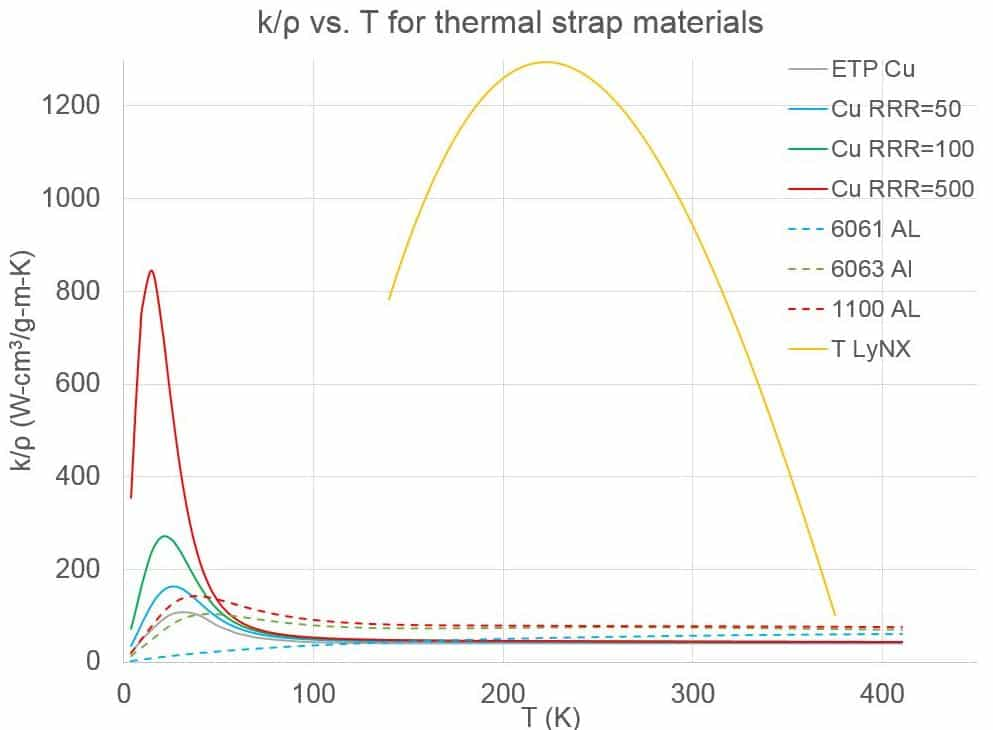
\includegraphics[height=0.3\textwidth]{Media/tcs_strap_01.JPG}\label{fig:tcs_strap11}}\qquad\qquad
	\subfloat[Example of a thermal strap, \cite{ref_tcs_01}.]{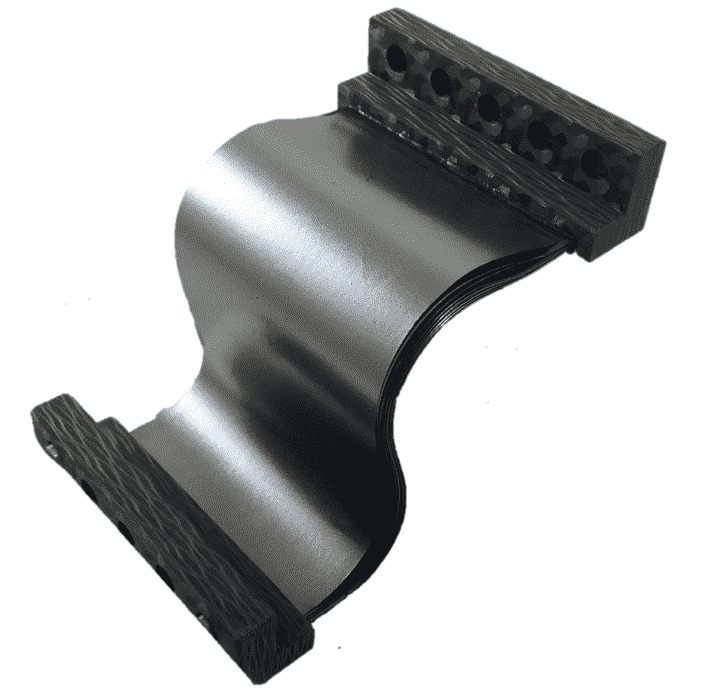
\includegraphics[height=0.2\textwidth]{Media/tcs_strap_02.png}\label{fig:tcs_strap12}}
	\caption{Carbon-based thermal strap \textit{LyNX}\textsuperscript{\tiny\textregistered}.}
	\label{fig:tcs_strap01}
\end{figure}


The camera, exposed on a mast, will be heated by a seperate, light weight Radioisotope Heater Unit (RHU), which has  been used during several NASA missions \cite{ref_tcs_02}.
For the insulation, the material \textit{Aerogel} will be applied, which has a very low heat conductivity (0.016 - 0.03\ $\frac{\W}{\m \K} $) as well as a low density (5 - 200\ $\frac{\kg}{\m^3}$) and has also been used in space applications \cite{ref_tcs_03}.

A surface finishing with an low emisivity for low heat emisivity is necessary.
For the most componets, a cost-efficient surface polishing is applicable.
The camera will get a special white paint with a high absorptivity to gather the  sun light.

But there is also a risk of overheating, because of the lack of heat convection.
This circumstance concern the engines and also the camera.
To get rid of the extensive heat and to prevent damage of the components special bi-metallic heat switches (see \autoref{fig:tcs_switch01}) will be  placed between the application and the connection interface.
These switches change their heat conductivity beyond a certain temperatur due to the expansion of the disk (see \autoref{fig:tcs_switch21}).
It was assumed, that the toggle temperatur can be adapted by increasing the disk height.
The influence of the changed disk stiffens on the contact pressure and therefore the heat conductivity was neglected for this study.
The measured heat conductivity characterisitc was divided in three linear sections (\autoref{fig:tcs_switch22}), to enable a simple modelling in the upcoming thermal calculation.

\begin{figure}[h]
	\centering
	\subfloat[Closed switch, high heat conduction.]{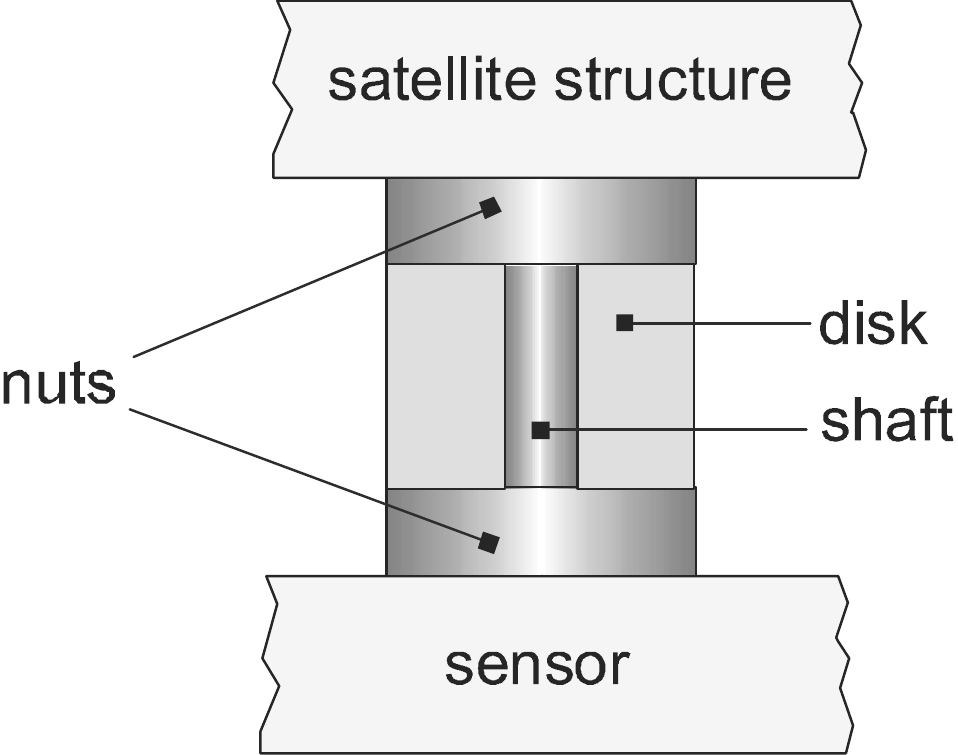
\includegraphics[height=0.18\textwidth]{Media/tcs_switch_01.png}\label{fig:tcs_switch11}}\qquad\qquad
	\subfloat[Open switch, reduced heat conduction.]{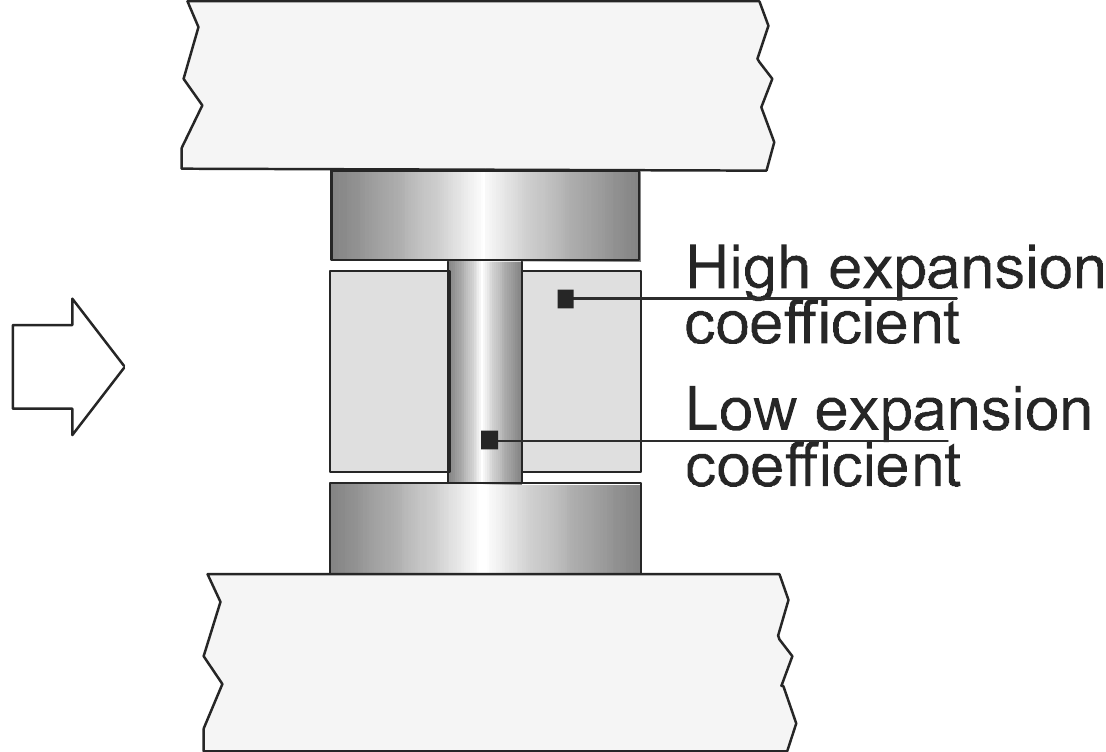
\includegraphics[height=0.18\textwidth]{Media/tcs_switch_02.png}\label{fig:tcs_switch12}}
	\caption{Bi-metallic heat switch, \cite{ref_tcs_04}.}
	\label{fig:tcs_switch01}
\end{figure}

\begin{figure}[h]
	\centering
	\subfloat[Comparison between data and theory (experimental results), \cite{ref_tcs_04} ]{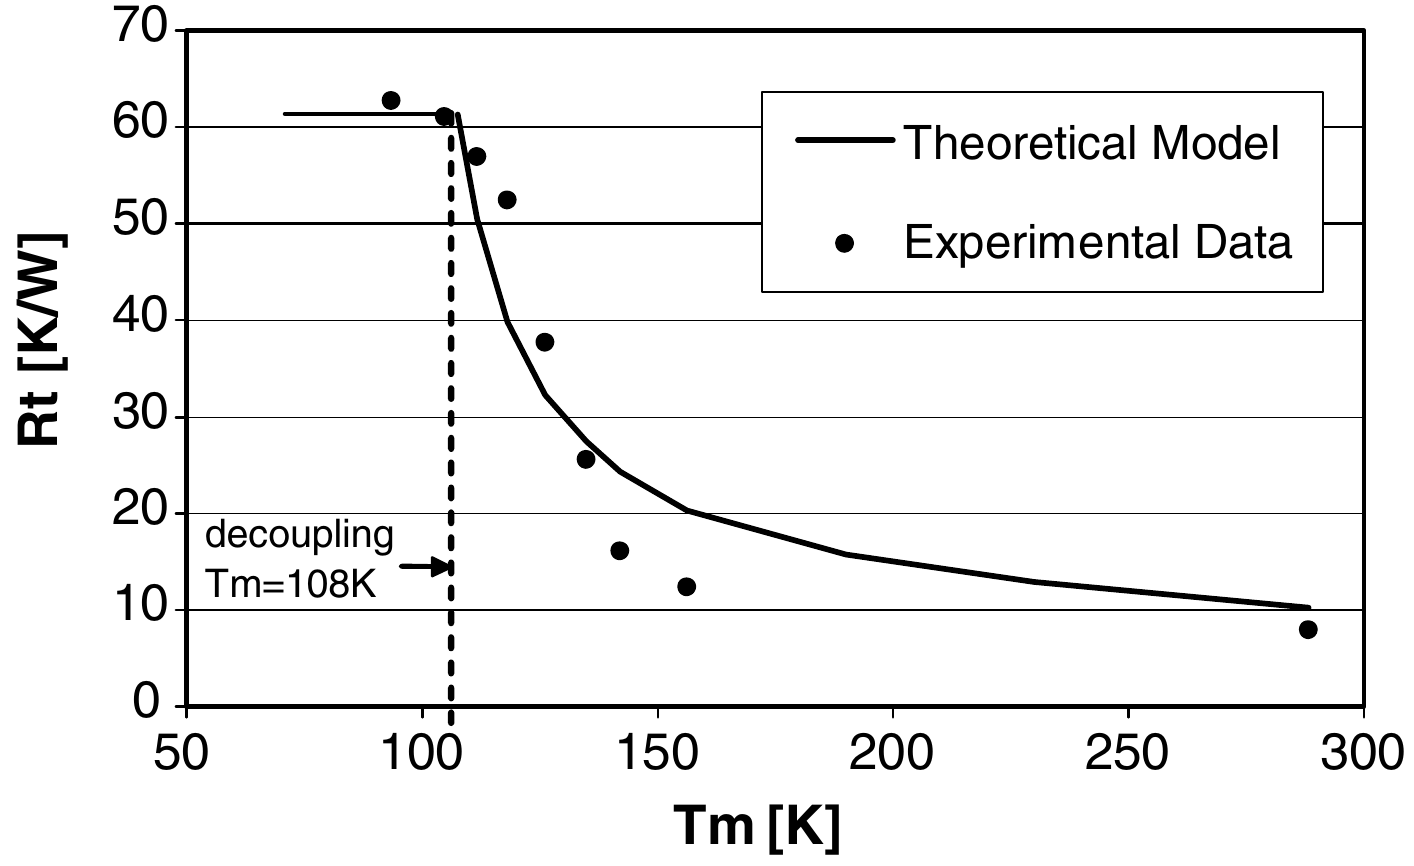
\includegraphics[height=0.22\textwidth]{Media/tcs_diag_orig.png}\label{fig:tcs_switch21}}\qquad
	\subfloat[Linearised characteristic of bi-metallic heat switch. ]{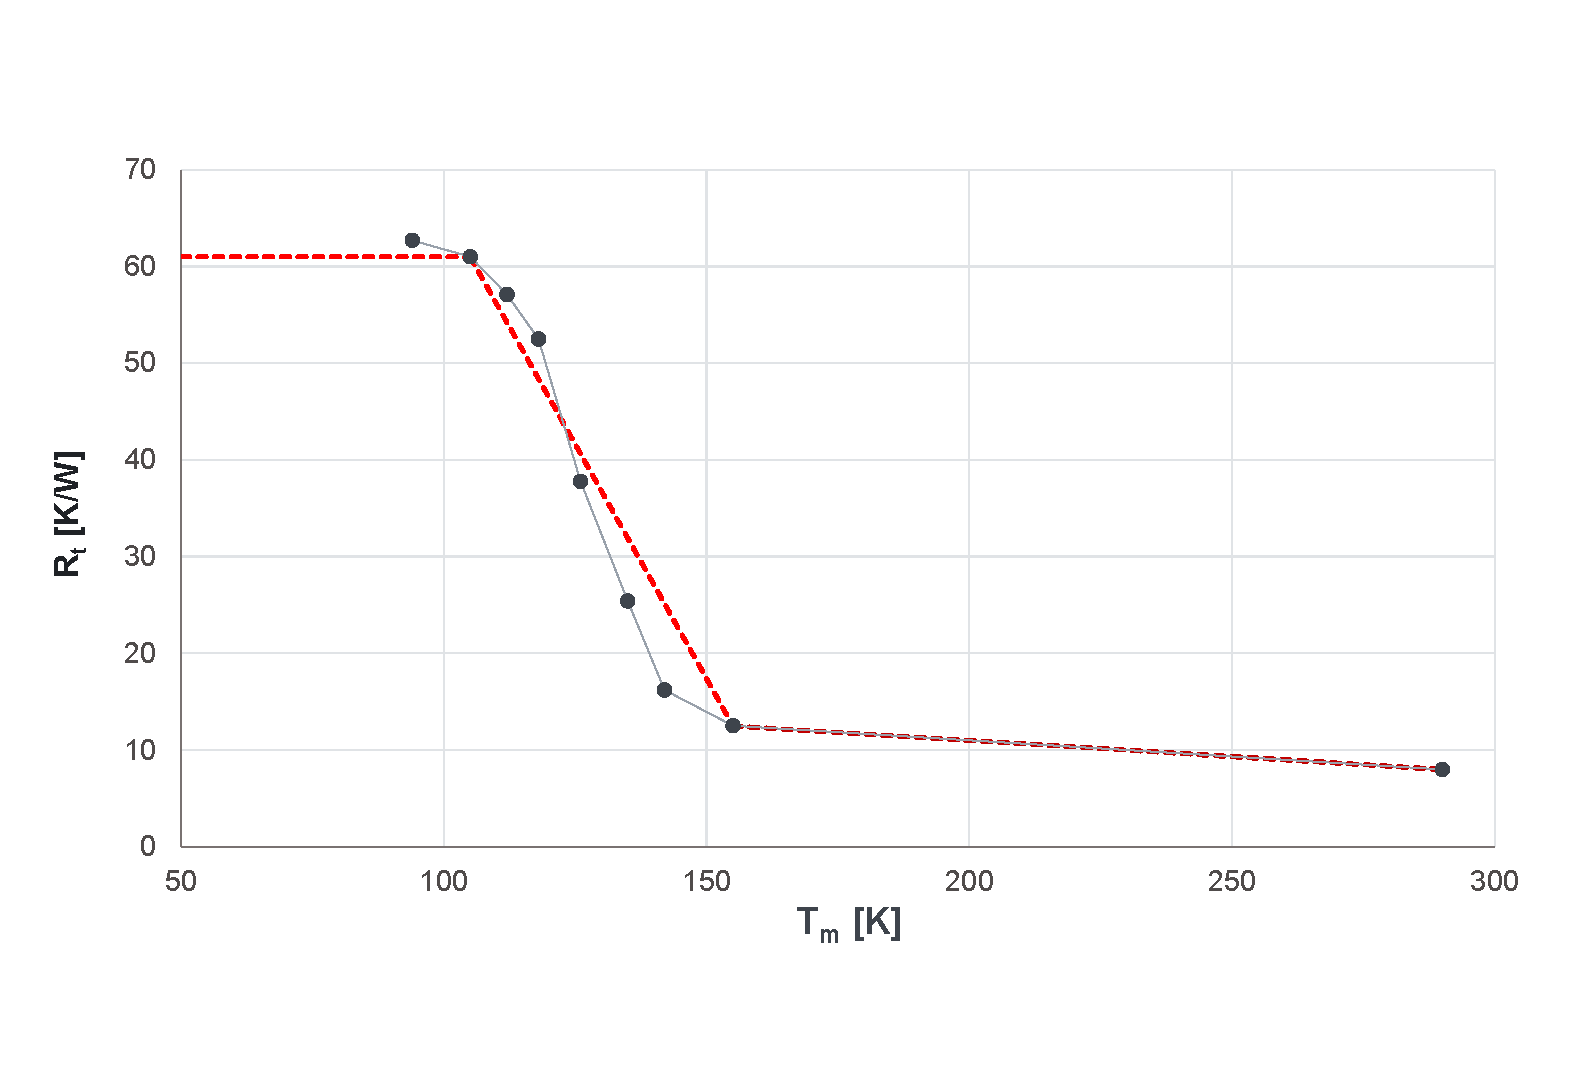
\includegraphics[height=0.22\textwidth]{Media/tcs_diag_lin}\label{fig:tcs_switch22}}
	\caption{Change of the heat switch conductivity $R_t$ over the mean temperature $T_M$.}
	\label{fig:tcs_switch02}
\end{figure}

\subsection{Thermal Network}
A thermal analysis was performed in order to get
\begin{itemize}
	\item the dimension of the insulation and heat straps,
	\item the necessary amount of RHUs and heat switches,
	\item the required surface finishing and
	\item the suitable choice of material.\\
\end{itemize}

For that, a thermal network with ten nodes was derived from the rover, shown in \autoref{fig:tcs_network}.
At the intersection of the steering and drive engien, two additional nodes were defined to calculate the heat flow.

\begin{figure}[H]
	\centering
	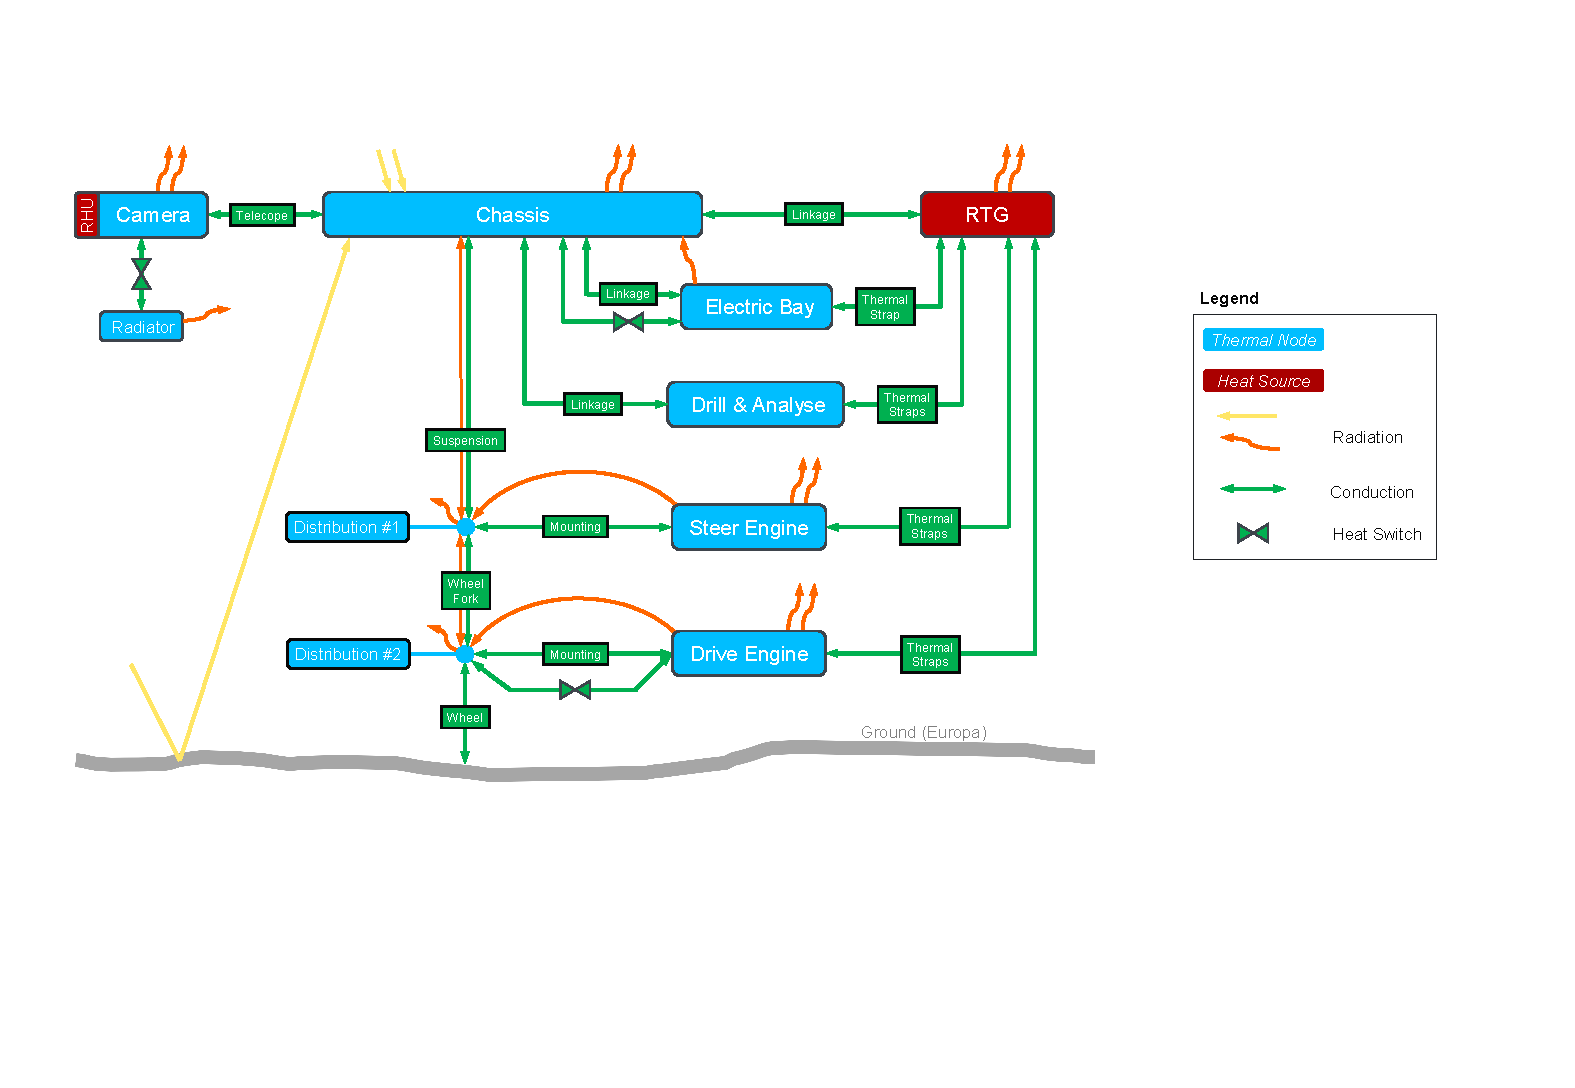
\includegraphics[width=0.85\textwidth]{Media/tcs_network}
	\caption{Thermal network of the rover.}
	\label{fig:tcs_network}
\end{figure}

On the basis of the thermal network, the heat energy equlibrium for each node was defined (see \appref{sec:app_tcs_01}).
The calculation were considered as a quasi-static analysis, were the component temperatures stay constant, $\frac{\dd T}{\dd t}=0$.
Due to the early state of the rover, simplifications and asumptions for the analysis were made.
\begin{itemize}
	\item The convection was neglected due to the thin atmosphere.
	\item The whole electrical power of the components will be dissipated into heat.
	\item A variation of $\pm 20\%$ for the emisivity and absorpsivity values was considered, if applicable (seet \autoref{tab:tcs_surface}).
	\item The heat as a result of retardation radiation inside the shielding was neglected.
	\item No dicrete nodes for the radar, hazcams and deployment engines were considered. Their heat will be lead into the chassis.
\end{itemize}


\subsection{Analysis}
The thermal analysis was perfomred as an Excel calculation, which can be found in the corresponding folder of Team 3.
The calculation sheet offers the possibility to adapt and customise input values and dimension.
The major driving load cases are the  hot and the cold cases, where the maximum and minimum temperatures of the rover components will be reached.
For that, the most powerful components were set to operating mode at once or only the minium requred components were turned on, respectively.
The emisivity and absorptivity were adjusted to fulfil the cases.
There were further load cases defined in order to cover important mission cases.

\subsection{Results}
The resulting temperatures for each node for the hot and cold cases  are listed in \autoref{tab:tcs_temp}.
The temperature margins for uncertainties, acceptance tests and qulification tests were considered with 5 K each, $\pm$15 K in total.
The corresponding temperatures are listed in \autoref{tab:tcs_temp}.
All temperature lay betwenn their limits without using a heater.
Nevertheless, heaters were considered for the power calculation, see \autoref{sec:EPS}.

\begin{table}[htb]
	\centering
	\caption{Temperature results in K of thermal analysis, including a margin of $\pm15\ \K$.}
	\begin{tabular}{l@{\qquad\qquad}cc@{\qquad}|@{\qquad}cc}
		\hline
		Components & \multicolumn{4}{c}{Load Case}   \\ \hline
		& \multicolumn{2}{l}{Hot case} & \multicolumn{2}{l}{Cold case} \\
		& $0$\ K & $+15$\ K & $0$\ K & $-15$\ K \\ \hline
		RTG  & 380 & 395 & 350 & 335   \\
		Electric Bay & 310 & 325 & 261 & 246  \\
		Drill \& Analyser & & & &  \\
		Camera & & & &  \\
		Steering Engine & & & &  \\
		Drive Engine & & & &  \\   \hline
	\end{tabular}
	\label{tab:tcs_temp}
\end{table}

In a furher step, a more detailed analysis should to be carried out with the Finite-Element-Method to identify the correct heat and temperature distribution.
The FE results could be used to verify and adjust the analytical analysis to get a helpful tool for fast thermal calculation to evaluate different materials or desings in the further development phases.
%A transient analysis could also help to optimise the insulation design.


\cleardoublepage